
%(BEGIN_QUESTION)
% Copyright 2015, Tony R. Kuphaldt, released under the Creative Commons Attribution License (v 1.0)
% This means you may do almost anything with this work of mine, so long as you give me proper credit

\noindent

\vskip 5pt

\vskip 5pt
\begin{center}
\textbf{Styresystemer -- Nivå 1 }
\vskip 5pt 
\textbf{Arbidsoppdrag på Egen PC}
\vskip 5pt 
	\textbf{Optimalisering av simulerte prosesser}
\end{center}

\textbf{Introduksjon}
I Dette arbeidsoppdraget  skal du jobbe med et \href{https://rfka-my.sharepoint.com/:u:/g/personal/fred-olav_mosdal_skole_rogfk_no/EdYP_MBtF1hIv2zqvzwtseMBLPwboQBdzCetAxSY83kwLw?e=PAZiw7}{Reguleringsundervisnings prosjekt for codesys}. \\

Du må starte dette kokumentet i Codesys og gjennomføre:
\begin{itemize}[noitemsep]
\item Repitisjon Z\&N
\item Oppgaven Her skal du optimalisere alle prosessene med følgende metoder
\begin{itemize}[noitemsep]
\item Tims rule of tumb
\item Z\&N
\item Skogestads metode
\end{itemize}


\end{itemize}

%$$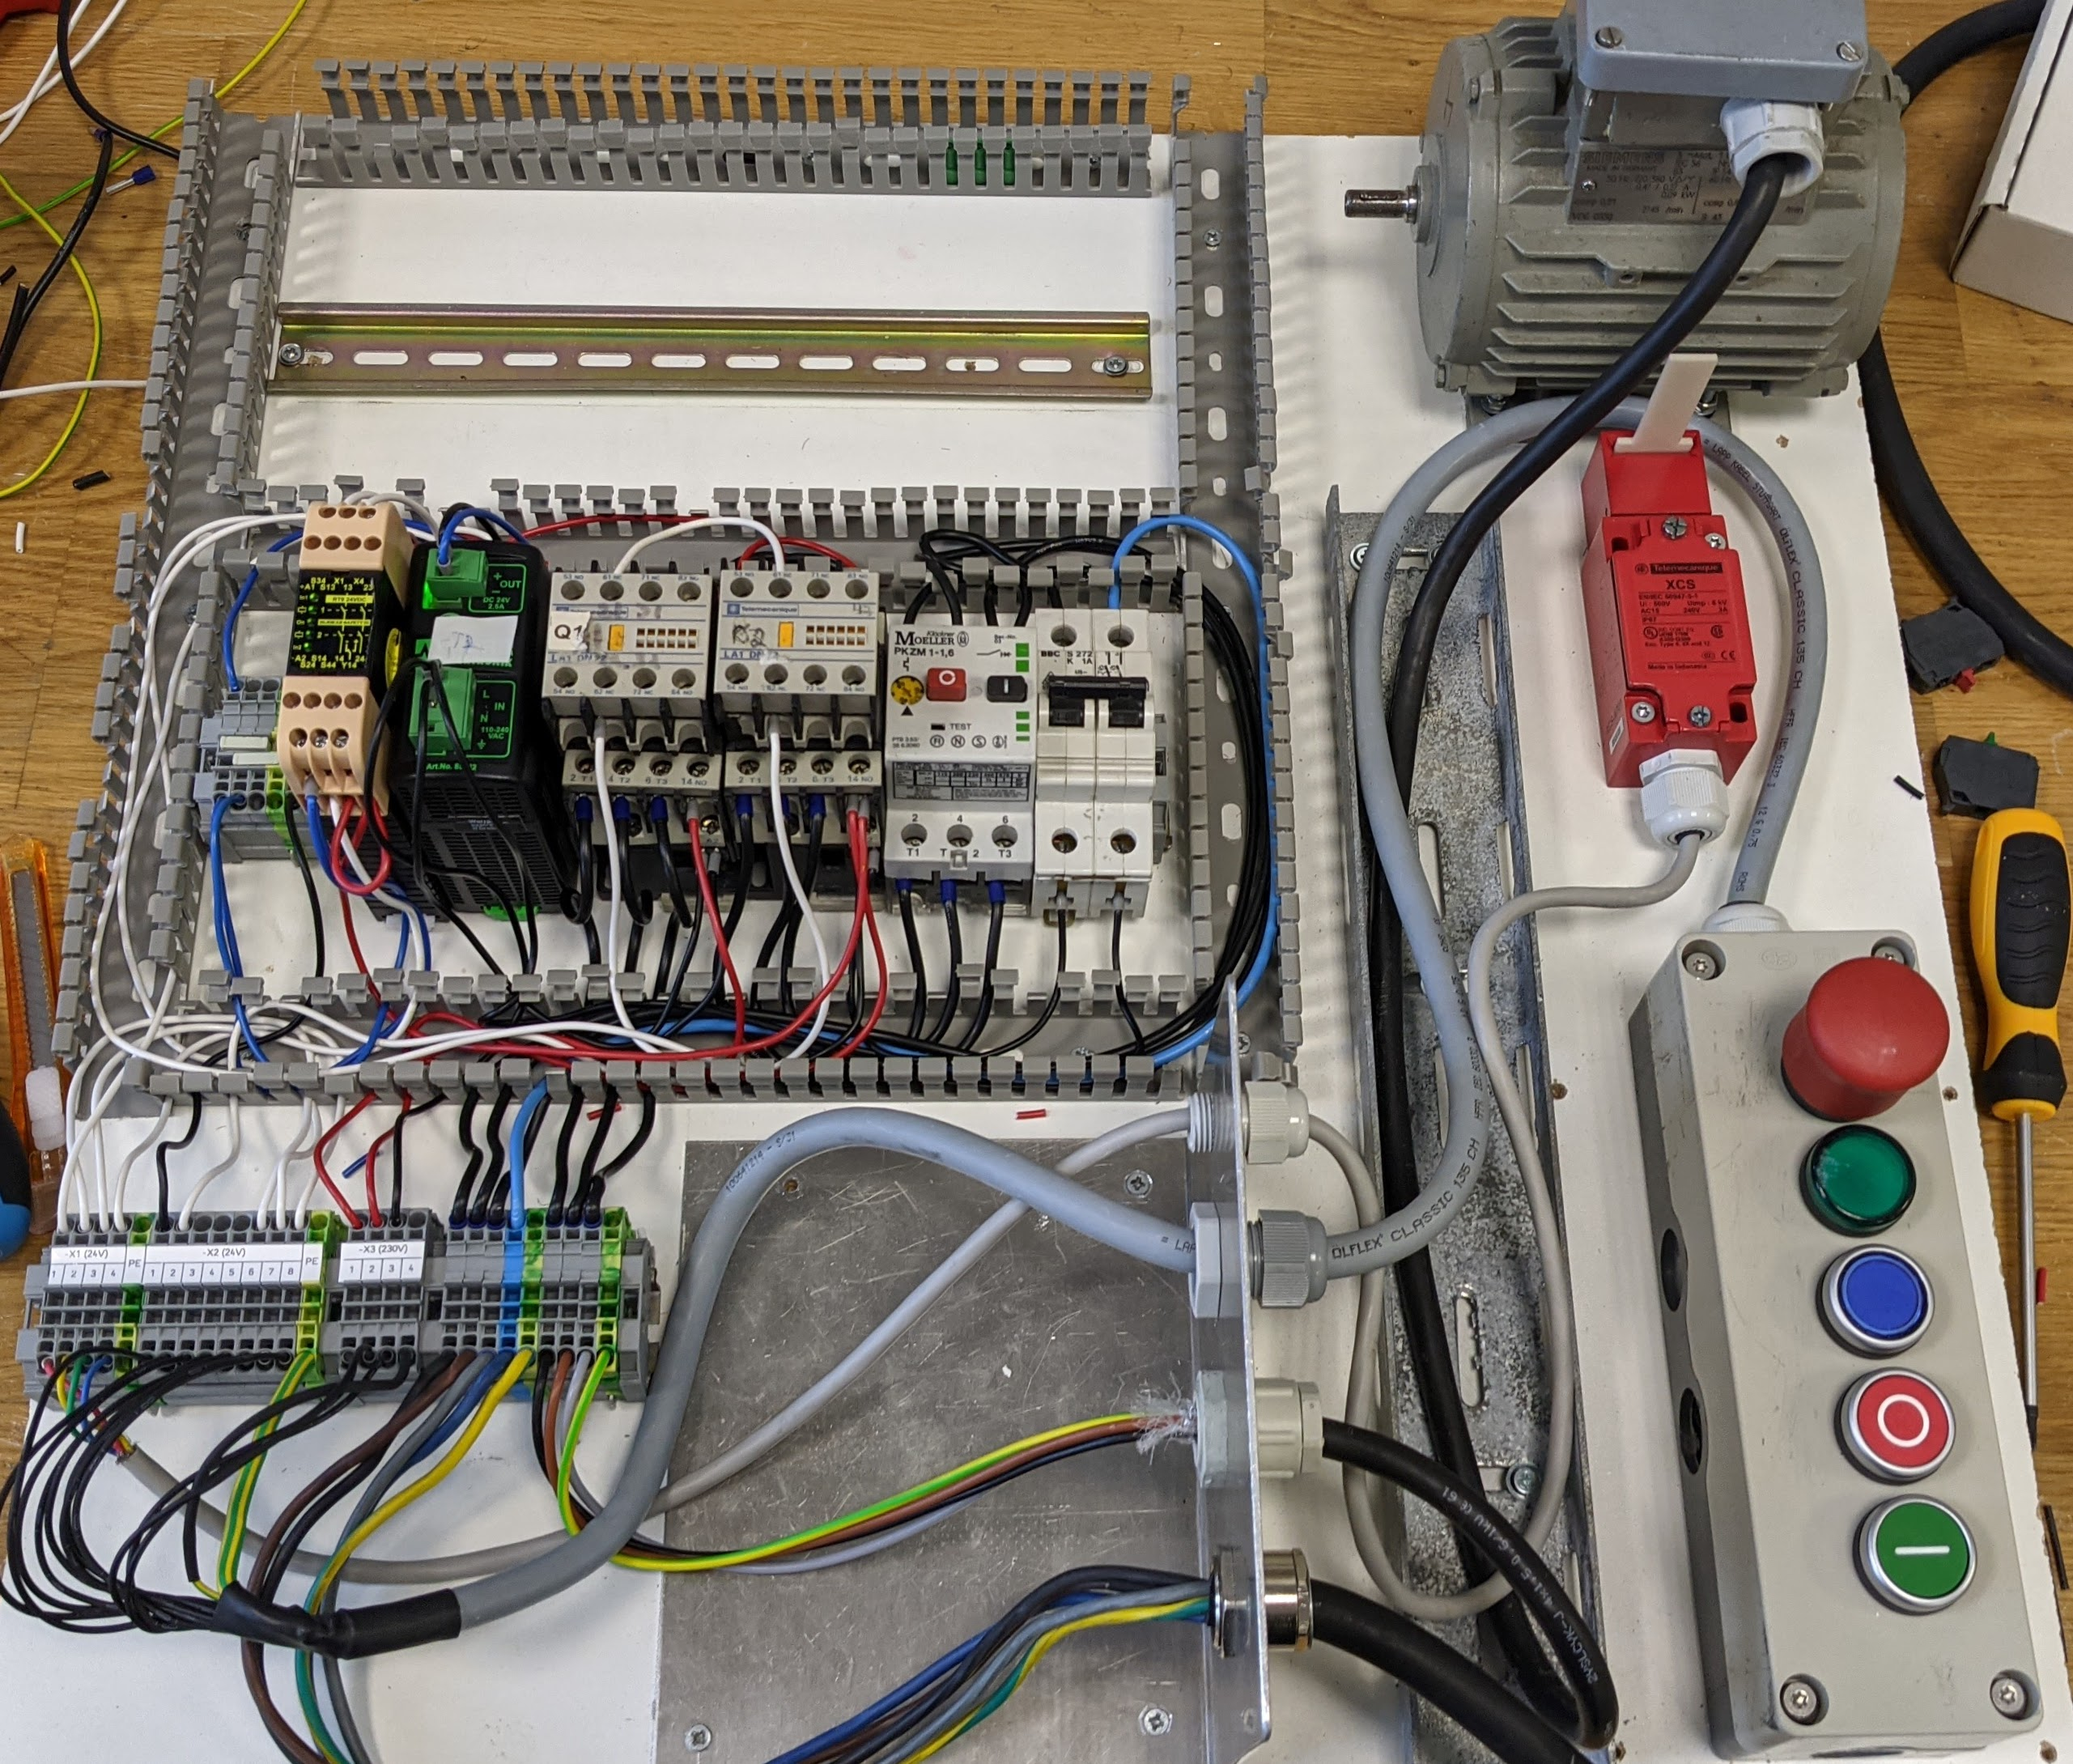
\includegraphics[width=13cm]{i04821x01.jpg}$$\\

\vskip 10pt 
\textbf{Teorioppgaver}

\vskip 5pt 

\vskip 10pt 
\textbf{Planlegging}


\vskip 10pt 
\textbf{Gjennomføring}

\vskip 10pt 
\textbf{Dokumentasjon}

Lag et dokument som viser hvordan du gikk frem for å optimalisere med de ulike metodene. 
Beskriv hvordan du planlegger, gjennomfører og dokumenterer denne jobben. 


















\underbar{file i04853}
\vfil \eject
%(END_QUESTION)





%(BEGIN_ANSWER)


%(END_ANSWER)





%(BEGIN_NOTES)


%INDEX% Arbeisdoppdrag, Regulering, Nivå 1, Egen PC, Innregulering med Tims, Z&N og Skogestads

%(END_NOTES)


